\subsection{Observation and latent-process model}

    The next inverse problem explicitly separates a population trajectory,
    correlated departures from that trajectory, measurement error, and
    posterior parameter uncertainty \citep{stuart2010inverse}. Time is expressed
    as \(s=(t-t_0)/12\), using a fixed scale across all training cutoffs.
    Responses retain their original numerical units. The physical units
    inherited by earlier figures have not been independently confirmed.

    Let \(m_\theta\) be a logistic population median with an uncertain initial
    value \(x_0\), rather than a first observation fixed without error:
    \[
        m_\theta(s)
        =\frac{K}{1+(K/x_0-1)\exp(-\rho s)},
        \qquad K>x_0>0,\quad \rho>0.
    \]
    The growth rate on the original time scale is \(r=\rho/12\).
    For each trial, the proposed model is
    \[
        \log(Y_i^{[j]}/y_{\rm ref})
        =\log(m_\theta(s_i)/y_{\rm ref})+U_j(s_i)+\varepsilon_i^{[j]},
        \qquad
        \varepsilon_i^{[j]}\sim\mathcal N(0,b^2),
    \]
    where \(y_{\rm ref}=1\) in the original response units and
    \[
        dU_j=-\lambda U_j\,ds+\sqrt{2\lambda}\,a\,dW_j(s),
        \qquad U_j(0)\sim\mathcal N(0,a^2).
    \]
    The trial processes and measurement errors are conditionally independent
    across trials. The OU component represents correlated deviations in log
    response; the logistic law governs the population median. The independent
    observation-error comparator sets \(a=0\) and omits the irrelevant
    correlation-rate parameter.

    The OU transition is available exactly
    \citep{sarkka2019applied}. Marginalizing the latent states gives, for each
    trial, a Gaussian log-response covariance
    \[
        C_{ik}=a^2\exp(-\lambda|s_i-s_k|)+b^2\delta_{ik}.
    \]
    Thus the parameter likelihood is evaluated by a Cholesky factorization of
    \(C\), independently of any Euler simulation step. The Jacobian
    \(-\sum_{i,j}\log Y_i^{[j]}\) is retained when expressing the density on
    the original response scale. An independent scalar Kalman implementation
    verifies this covariance likelihood numerically. Initial observations are
    included in the likelihood and their latent uncertainty is propagated.

\subsection{Declared priors and computational checks}

    The transformed coordinates are
    \[
        z=\left(
            \log(x_0/y_{\rm ref}),\;
            \log(K/x_0-1),\;
            \log\rho,\;\log\lambda,\;\log a,\;\log b
        \right).
    \]
    Their independent normal prior means and standard deviations are
    \[
        \mu_z=\log(10,3,0.5,0.5,0.03,0.03),\qquad
        d_z=(1.5,1,1.25,1.25,1,1).
    \]
    These are proper exploratory priors in declared numerical units. They are
    analyst choices, not externally elicited physical information. They are
    fixed across time cutoffs and are not fitted to held-out scores. The
    choices follow the earlier exploratory analysis; these retrospective
    holdouts do not constitute an untouched validation study. The
    sensitivity analysis multiplies both noise prior medians by \(1/2\) or
    \(2\), leaving the likelihood and other priors fixed. Priors are specified
    on \(z\), so no additional transformation Jacobian is applied to its
    normal prior density. The observation-only comparator retains coordinates
    1, 2, 3, and 6 with the same reference priors.

    Four Metropolis chains use adaptation during warmup only. The subsequent
    proposal kernels are fixed, symmetric Gaussian mixtures and use the exact
    marginalized likelihood. Local curvature initializes the proposal; the
    posterior target remains the full nonlinear parameter posterior.
    Rank-normalized and folded split \(\widehat R\), bulk ESS, and tail ESS
    are monitored for transformed and reported parameters
    \citep{vehtari2021rank}. The computational acceptance criteria are
    \(\widehat R<1.01\) and both ESS measures at least 400. Longer runs are
    used when needed; exact settings are recorded per experiment. These finite
    diagnostics do not prove convergence. Analytic Gaussian sampler tests,
    covariance-versus-Kalman likelihood checks, and exact conditional-variance
    tests provide independent implementation checks.

\subsection{Posterior prediction and uncertainty decomposition}

    For each retained parameter vector, Gaussian conditioning gives the latent
    predictive mean and covariance from training data alone. Measurement
    variance \(b^2\) is then included for a new response. The posterior
    predictive distribution integrates both over these latent states and over
    the parameter posterior. On the original scale it is a mixture of
    lognormal distributions. The saved mean curves use finite posterior-subset
    averages of conditional lognormal means, including the variance correction.
    The unbounded noise-SD priors give an infinite full response-scale
    predictive mean, as established in Section~\ref{sec:predictive-moments}.
    These finite averages and their historical RMSE/bias scores must therefore
    be interpreted as finite-mixture diagnostics. Pointwise quantiles solve
    the posterior-mixture CDF, avoiding
    additional Monte Carlo noise from simulating observation errors.

    For a future log response, the law of total variance gives
    \[
        \operatorname{Var}(\log Y_*\mid D)
        =\operatorname{Var}_{\theta\mid D}(\mu_\theta)
        +\mathbb E_{\theta\mid D}[V_{U,\theta}]
        +\mathbb E_{\theta\mid D}[b^2].
    \]
    The first term measures variation of the conditional mean across
    parameters; the second is conditional latent-state uncertainty; the third
    is measurement error. Dependence among inferred parameters is retained by
    joint posterior draws. A credible band for \(m_\theta\) summarizes the
    population median and has a different interpretation from a predictive
    interval for a new noisy observation.

% Generated by scripts/summarize_bayesian_observation.py; do not edit manually.
\begin{table}[htbp]
\centering
\caption{Bayesian time holdouts. Intervals integrate parameter, latent-state, and measurement uncertainty.}
\label{tab:bayesian-forecast}
\begingroup\small\setlength{\tabcolsep}{4pt}
\begin{tabular}{llrrrr}
\toprule
Model & Cutoff & RMSE & Coverage & Width & Marginal NLL \\
\midrule
IID & 108 & 2.1863 & 0.8667 & 5.7894 & 2.2310 \\
IID & 120 & 2.4573 & 0.6667 & 5.4563 & 2.4875 \\
IID & 132 & 2.7962 & 0.5556 & 5.2120 & 2.8763 \\
OU & 108 & 2.1564 & 0.8667 & 6.1572 & 2.1881 \\
OU & 120 & 2.4238 & 0.8333 & 5.7518 & 2.4081 \\
OU & 132 & 2.7692 & 0.6667 & 5.4952 & 2.7603 \\
\bottomrule
\end{tabular}
\endgroup
\end{table}
\begin{table}[htbp]
\centering
\caption{Noise-prior sensitivity for the latent OU model. Cutoff-weighted descriptive summaries reuse observations.}
\label{tab:bayesian-prior}
\begingroup\small\setlength{\tabcolsep}{4pt}
\begin{tabular}{lrrrr}
\toprule
Prior & RMSE & Coverage & Width & Marginal NLL \\
\midrule
Double noise prior & 2.4014 & 0.8333 & 6.0513 & 2.3793 \\
Half noise prior & 2.4116 & 0.7778 & 5.6955 & 2.4252 \\
Reference prior & 2.4110 & 0.8056 & 5.8566 & 2.4045 \\
\bottomrule
\end{tabular}
\endgroup
\end{table}
\begin{table}[htbp]
\centering
\caption{Full-data OU parameter posterior: marginal 90 percent credible intervals in the stated numerical units.}
\label{tab:bayesian-parameters}
\begingroup\small\setlength{\tabcolsep}{4pt}
\begin{tabular}{lrrr}
\toprule
Parameter & Median & 5th percentile & 95th percentile \\
\midrule
Initial median $x_0$ & 14.16014 & 13.68362 & 14.66370 \\
Capacity $K$ & 48.01205 & 47.17744 & 49.04975 \\
Rate $r$ & 0.04557 & 0.04267 & 0.04835 \\
Latent SD $a$ & 0.02764 & 0.00805 & 0.04465 \\
Measurement SD $b$ & 0.02658 & 0.00746 & 0.03939 \\
Correlation time $12/\lambda$ & 13.97064 & 3.27227 & 70.68001 \\
\bottomrule
\end{tabular}
\endgroup
\end{table}


    The cutoff-weighted reference OU coverage is 0.8056, with
    RMSE 2.4110 and mean predictive width 5.8566. The
    observation-only Bayesian comparator has coverage 0.7222.
    For the same OU model with coefficients fixed at their marginal posterior
    medians, coverage is 0.6944; this isolates a plug-in comparison
    within that model, rather than attributing every change from the earlier
    neural fits to parameter uncertainty alone. Noise-prior sensitivity gives
    descriptive coverage ranging from 0.7778 to 0.8333.

    All reported runs meet the declared computational thresholds: the largest
    monitored $\widehat R$ is 1.0070, minimum bulk ESS is
    641, and minimum tail ESS is 444.
    These checks support finite-run numerical reliability, not model adequacy.
    The noise split and correlation time remain uncertain. The intervals in
    Table~\ref{tab:bayesian-parameters} are parameter credible intervals;
    the forecast bands in Figure~\ref{fig:bayesian-forecast} are observation
    predictive intervals. The original residual AIC/BIC scores are not used
    as Bayesian model evidence.

    All seven uncovered responses across the reference OU holdouts exceed
    their upper bounds. Mean observed-minus-predicted residuals increase from
    approximately 1.28 to 2.25 response units across the cutoffs. This pattern
    motivates investigation of structural underprediction, rather than a
    claim that parameter integration has resolved calibration. A predictive
    mixture integration check using 6000, 12000, and 24000 posterior draws at
    cutoff 132 leaves coverage unchanged; interval endpoints shift by at most
    approximately 0.012 response units relative to the 6000-draw calculation.

    The holdouts still reuse 15 distinct scalar observations across 36 forecast
    entries. A near-nominal aggregate rate would not establish calibration on
    independent future experiments. The Bayesian extension is retained as an
    exploratory observation-model comparison, and REV-07 remains open until
    predictive adequacy is established with stronger validation.

\begin{figure}[htbp]
    \centering
    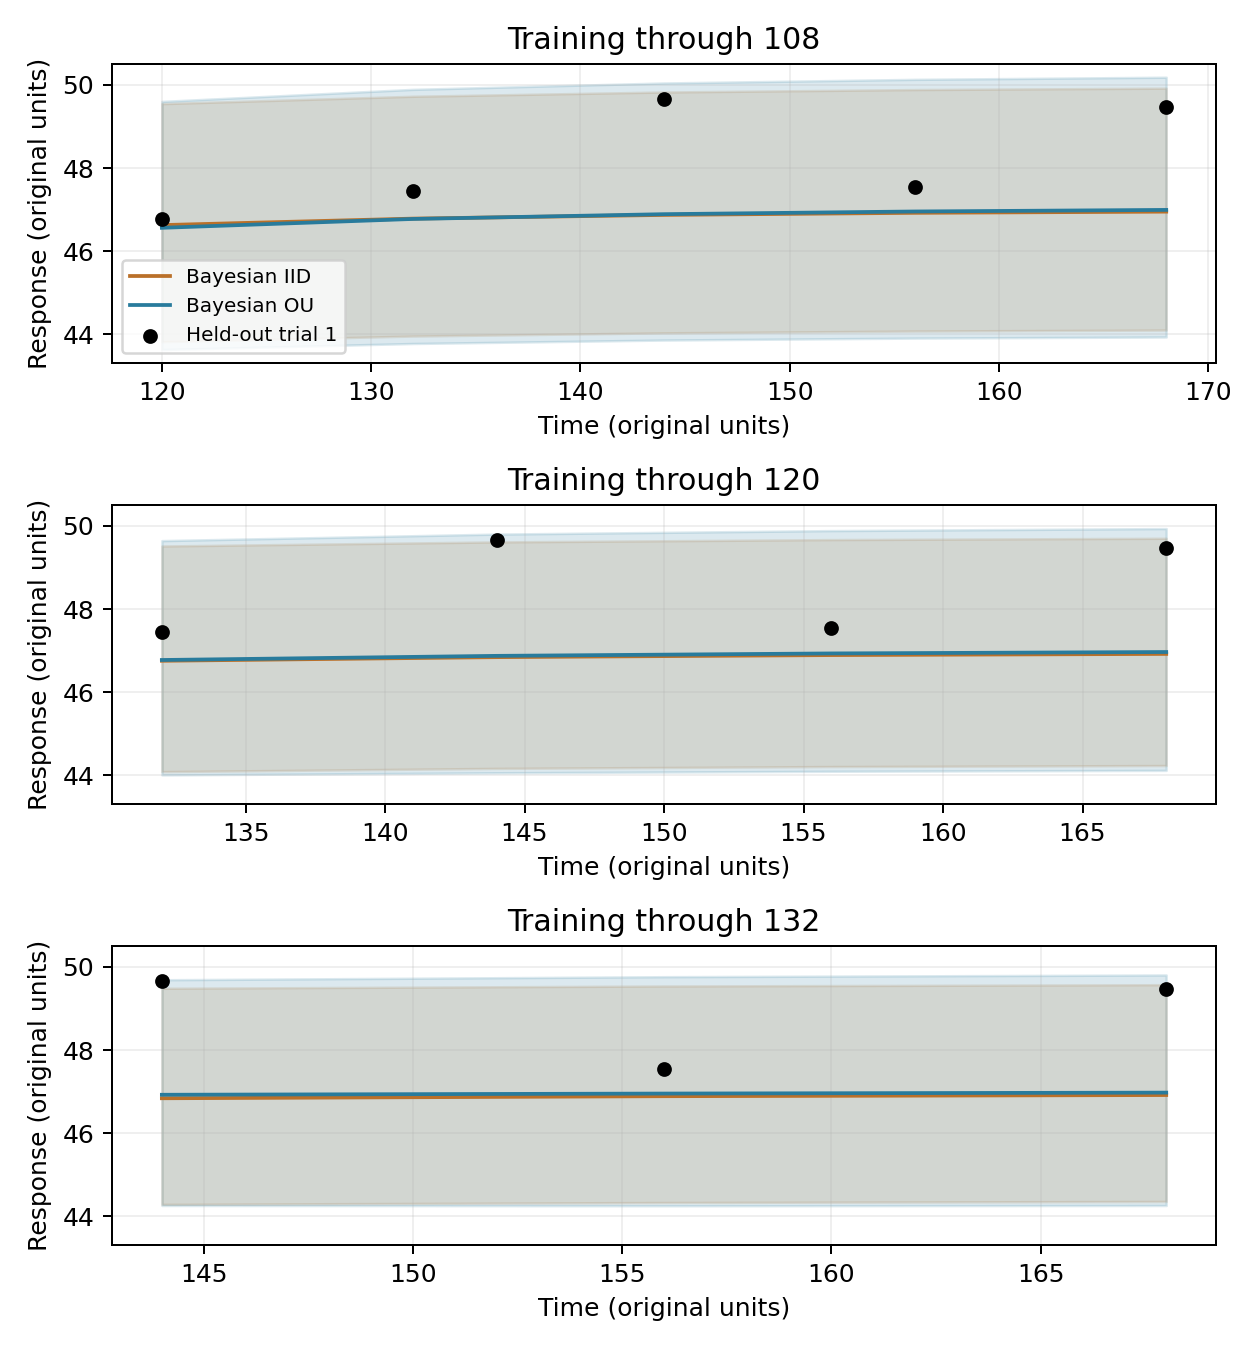
\includegraphics[width=\textwidth]{../results/bayesian/forecast_comparison.png}
    \caption{Posterior predictive means and central 90 percent observation
    intervals for trial 1. Black markers are held-out responses. Metrics use
    all three trials; intervals integrate the parameter posterior.}
    \label{fig:bayesian-forecast}
\end{figure}
\begin{figure}[htbp]
    \centering
    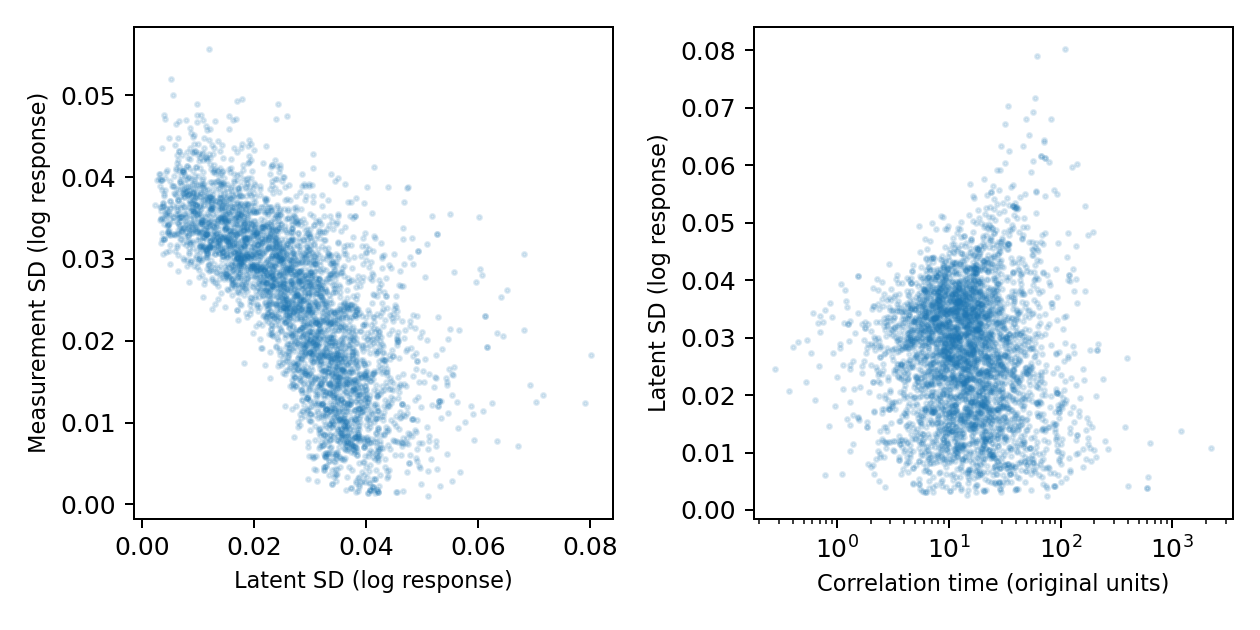
\includegraphics[width=0.9\textwidth]{../results/bayesian/noise_identifiability.png}
    \caption{Joint posterior noise and correlation parameters for the full-data
    OU model. Correlation of noise components and a broad correlation-time
    range limit a mechanistic interpretation of their separate estimates.}
    \label{fig:bayesian-identifiability}
\end{figure}

